\documentclass[10pt, a4paper]{report}

\usepackage[utf8]{inputenc}
\usepackage[portuges]{babel}
\usepackage{blindtext}
\usepackage{enumitem}
\usepackage{graphicx}
\usepackage{cite}

\title{Desenvolvimento de Sistemas de Software \\ \large{Mestrado Integrado em Engenharia Informática}}
\author{Luís Capa \\ A81960 \\ 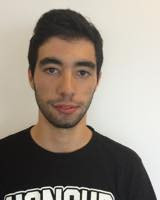
\includegraphics[width = 20mm]{luis}
	\and 
	Moisés Antunes \\ A82263 \\ 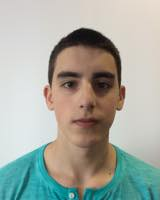
\includegraphics[width = 20mm]{moises}
	\and
	Pedro Capa \\ A83170 \\ 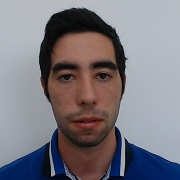
\includegraphics[width = 20mm, height = 25mm]{pedro}
}
\date{\today}

\begin{document}
\maketitle
\tableofcontents

\chapter{Introdução}\label{Intro}
Hoje em dia, os clientes das grandes marcas de automóveis têm a possibilidade de personalizar o carro da maneira como quiserem. Para tal, os clientes podem escolher peça a peça, escolher um pacote ou escolher configuração ótima em relação ao orçamento. O cliente não pode escolher todas as peças que quer, visto que há peças que são incompatíveis e outras que são obrigatórias. Os componentes na fábrica têm um stock, no caso de chegarem novas peças é necessário informar o sistema que chegaram novas peças e os carros que estão à espera dessas peças voltam para a fila de produção.

\chapter{Objetivos}\label{objetivos}
Esta unidade curricular tem o objetivo de mudar a forma como nós programamos, pois até agora sempre que recebiamos um projeto começava-se a escrever código. Para isso usou-se a linguagem UML para preparar a escrita do código de forma a cometer menos erros quer na criação de classes quer no objetivo do projeto em si. 
O relatorío tem o objetivo de clarificar o trabalho realizado no geral, bem como as suas partes.

\chapter{Trabalho realizado}\label{trabalho}
Para este trabalho foram criados alguns modelos UML como o modelo de dominio, UseCase e os diagramas de estado.
No "Visual Paradigm" foi criado um modelo de domínio que mostra as prinicipais relações entre entidades criadas para este problema. No mesmo programa foi criado o modelo de use cases. Este modelo mostra as principais interações entre os atores do sistema com o própio sistema. Nesta aplicação foram consideradas duas entidades que teriam diferentes estados, o carro e a peça. Para descrever as diferentes fases destas entidades foi criado para cada uma um modelo de estado.
O modelo de interface foi realizado no "NetBeans", uma vez que será essa a ferramenta usada para a implementação do projeto e é mais fácil de implementar a interface gráfica, porque tem um visualisador de classes interfaces que gera automaticamente o código dos componentes do swing, api de interfaces usada. A interface foi modelada de acordo com os Use Cases do projeto, uma vez que este indica que opções cada ator realiza no sistema.
\end{document}